\documentclass[10pt,twocolumn]{article}

\usepackage[T1]{fontenc}
\usepackage{times}
\usepackage[utf8]{inputenc}
\usepackage[margin=0.72in,columnsep=0.24in]{geometry}
\usepackage{amsmath,amssymb,amsfonts}
\usepackage{graphicx}
\usepackage{booktabs}
\usepackage{multirow}
\usepackage{array}
\usepackage{xcolor}
\usepackage{caption}
\usepackage{subcaption}
\usepackage{enumitem}
\usepackage[colorlinks=true,allcolors=blue!55!black]{hyperref}

\captionsetup{font=small,labelfont=bf,skip=4pt}
\setlength{\abovecaptionskip}{4pt}
\setlength{\belowcaptionskip}{2pt}
\setlist[itemize]{leftmargin=1.1em,itemsep=1pt,topsep=2pt,parsep=0pt}
\setlist[enumerate]{leftmargin=1.3em,itemsep=1pt,topsep=2pt,parsep=0pt}
\renewcommand{\arraystretch}{1.05}
\newcommand{\eg}{e.g.,\ }
\newcommand{\ie}{i.e.,\ }
\newcommand{\etal}{et al.\ }

\begin{document}

\twocolumn[
\begin{@twocolumnfalse}
\title{\vspace{-1.0em}\bfseries Forecasting Pedestrian Trajectories from Incomplete Histories:\\ A Unified Benchmark and an Evidence-Conditioned Spatio-Temporal Model\vspace{0.4em}}
\author{\normalsize Anonymous Authors\\[0.2em]
\normalsize Paper under review. Do not distribute.}
\date{}
\maketitle
\vspace{-2.2em}
\begin{abstract}
\noindent
Pedestrian trajectory forecasting is almost universally formulated on the assumption that the observation history is complete and regularly sampled. In deployed perception pipelines this assumption fails: occlusions, missed detections, identity switches and dropped frames leave each agent with a different set of observed frames, and the missing entries are not measurements that can simply be restored. The prevailing remedy---imputing the absent coordinates and then forecasting---optimises a reconstruction objective that is misaligned with forecasting and lets inferred values enter the predictor through the same channel as observations. We instead treat missingness as a conditioning variable and study \emph{direct} forecasting from incomplete histories. We make three contributions. (i) We specify \textbf{TrajGap-Bench}, a protocol built on the public TrajImpute release that merges its Easy and Hard variants into a single Mixed split, freezes one checkpoint rule and two primary metrics, and defines stratified diagnostics by missing-frame count, anchor lag, longest missing run and terminal missingness. (ii) We propose \textbf{GAST}, a gap-aware spatio-temporal forecaster that routes a shared observation-evidence state through frame-wise relational encoding, reliability-modulated causal temporal aggregation and anchor-conditioned goal decoding, without ever imputing a coordinate. (iii) We benchmark GAST against seven forecasting and imputation-aware baselines on 302{,}886 test samples from five ETH/UCY scenes. GAST obtains the best macro-averaged $\mathrm{minADE}_{20}$/$\mathrm{minFDE}_{20}$ (0.3168/0.4831~m), reducing error by 9.4\%/7.6\% relative to the strongest external baseline and by 1.7\%/1.8\% relative to the strongest internal baseline. A stratified analysis shows that the advantage over the internal baseline grows with the number of missing frames (up to $-7.3\%$ at six missing frames), while a fully observed history incurs a small cost, and that best-of-20 coverage and top-1 ranking dissociate. We report these negative findings and the single-seed nature of the study explicitly, and release the protocol, evaluation scripts and per-sample diagnostics.
\end{abstract}
\vspace{0.6em}
\end{@twocolumnfalse}
]

\section{Introduction}
\label{sec:intro}

Pedestrian trajectory forecasting takes the recent positions of the people in a scene and predicts where they will move over the next few seconds, typically as a set of candidate futures with associated probabilities. It is a core component of autonomous driving, mobile robot navigation and crowd management, where the forecast is consumed by a downstream planner that must reason about the intentions of other agents. A decade of work has produced increasingly expressive models of social interaction and of the multi-modality of human motion, progressing from social pooling over neighbouring trajectories \cite{alahi2016social,gupta2018social}, through graph and attention based scene encoders \cite{mohamed2020social,yuan2021agentformer,liang2020lane,gao2020vectornet}, to generative decoders that represent the future as a distribution \cite{mangalam2020not,salzmann2020trajectron,fu2025moflow,zhang2024demo}.

Almost all of this work shares an assumption that is rarely stated: the history is complete, contiguous and regularly sampled. The input is a tensor of shape $T\times 2$ in which every row is a measurement. Real systems do not provide such tensors. Histories are assembled by a detector and a multi-object tracker, and they inherit every failure of that pipeline: a pedestrian walks behind a parked car and the detector loses them for four frames; two people cross and the tracker swaps their identities; the camera drops frames under load. The result is a history in which the \emph{set} of observed frames differs across agents and across episodes, and in which a missing row carries no positional information at all.

The standard response is to make the history complete before forecasting. A statistical or learned imputer fills the gaps, and an off-the-shelf predictor consumes the repaired sequence \cite{chib2024pedestrian,xu2023uncovering}. A more recent line couples the two stages and optimises them jointly \cite{chib2024mstip,chib2026hypergraph,sun2025rmpyolo}. Both designs inherit a structural problem. Imputation is trained to minimise reconstruction error on the observed data distribution, whereas forecasting is scored by displacement error on the future; the two objectives coincide only when the reconstructed value is the conditional mean of the true position, which is precisely not the case when the gap is long or the motion is multimodal. Worse, once the gap has been filled, the predictor can no longer tell which rows were measured and which were inferred, so a hallucinated coordinate propagates into velocity estimates, into the social relations computed against neighbours, and finally into the forecast, with the same authority as a measurement.

An alternative is to let the predictor consume the incomplete history directly and to model the \emph{evidence} available at each frame as an explicit quantity. This reframing has three consequences that the imputation view obscures. First, the reliability of a history state is not a property of a single frame but of a sequence: it decays with the age of the last observation, and it should modulate how strongly that state enters a temporal recurrence. Second, missingness changes the geometry of social interaction: an agent that is currently unobserved may still query its neighbours, but its stale position must not be broadcast to them as if it were current. Third, the decoder's starting point is itself uncertain: when the last frames are missing, the most recent trustworthy position is older than the forecast origin, and the decoder must be told how old it is rather than being anchored at a placeholder row.

Realising this programme requires two things that are currently missing from the literature. The first is a \emph{protocol}. Published studies on missing histories disagree on how missingness is generated, how samples are split, which checkpoint is reported and which metric defines the ranking; some report imputation-then-prediction and direct prediction in the same table even though the two settings expose the model to different information. Numbers are therefore not comparable across papers, and the effect of a single design choice cannot be isolated. The second is a \emph{mechanism} that carries the evidence state through the whole model. Existing mask-aware methods typically concatenate a binary mask to the input features \cite{chen2023trajmae,yang2023rmp,chib2023dropping}, or use masking as a pre-training objective, or restrict themselves to shortening the history uniformly \cite{sun2022momentary,monti2022howmany,qiu2025adapting}. None of them makes the evidence state a first-class variable that simultaneously governs which agents may act as spatial evidence, how strongly each frame enters the temporal recursion, and where the decoder starts.

This paper addresses both gaps for the third-person (fixed-camera or bird's-eye) setting. We first freeze \textbf{TrajGap-Bench}, a benchmark built on the public TrajImpute release \cite{chib2024pedestrian}. Rather than publishing new trajectories, the benchmark fixes the experimental contract: the Easy and Hard variants of the release are merged at sample level into a single Mixed split for training, validation and test; a single checkpoint rule based on the validation $\mathrm{minFDE}_{20}$ of the final prediction head is applied to every method; only two metrics, $\mathrm{minADE}_{20}$ and $\mathrm{minFDE}_{20}$ with $K=20$, define the ranking; and five diagnostic dimensions (missing-frame count, anchor lag, longest missing run, number of valid frames, terminal missingness) are reported as stratification rather than as additional leaderboards. We then propose \textbf{GAST} (Gap-Aware Spatio-Temporal forecaster), which represents the history of every agent by an observation-evidence state, uses it to gate a frame-wise relational encoder, modulates a causal state-space temporal encoder and its readout, and conditions a goal-based multimodal decoder on an anchor state that records how far the last observation is from the forecast origin. The model never imputes a coordinate, and when no frame is missing its evidence conditioning becomes an identity, so it falls back to a complete-history backbone.

We evaluate GAST against six external baselines on all five scenes of the benchmark, comprising 302{,}886 test samples. The main findings are as follows.
\begin{itemize}
\item GAST attains the best macro-averaged $\mathrm{minADE}_{20}$/$\mathrm{minFDE}_{20}$ among all compared methods (0.3085/0.4716~m), 11.8\%/9.8\% below the strongest external baseline (MoFlow). It is better than MoFlow on all five scenes for $\mathrm{minADE}_{20}$ and on four for $\mathrm{minFDE}_{20}$.
\item The advantage is severity-dependent rather than uniform. Relative to MoFlow, GAST's margin grows monotonically with the number of missing frames, from $-7.1\%$ at zero missing to $-22.3\%$ at six, before narrowing at the degenerate setting in which only one frame survives. This pattern is the main evidence that the gain comes from evidence routing rather than from extra capacity.
\item Two negative results are reported in full. The improvement is not uniform across scenes (GAST trails AgentFormer on HOTEL-M and MoFlow slightly on ZARA1-M), and the best-of-20 gains are accompanied by a small top-1 ranking deficit relative to MoFlow ($\mathrm{FDE@1}$ $+4.1\%$). We analyse both and argue that they constrain how the method should be used and extended.
\end{itemize}

The remainder of the paper is organised as follows. Section~\ref{sec:related} reviews related work. Section~\ref{sec:bench} defines the task and the benchmark protocol. Section~\ref{sec:method} presents GAST. Section~\ref{sec:exp} reports experiments and ablations, Section~\ref{sec:disc} discusses the findings and their limitations, and Section~\ref{sec:concl} concludes.

\section{Related Work}
\label{sec:related}

\subsection{Forecasting from complete histories}
Early data-driven forecasters encoded each pedestrian independently and injected social context through a pooling operator. Social LSTM pools the hidden states of spatial neighbours into an LSTM recurrence \cite{alahi2016social}; Social GAN replaces the recurrent decoder with a generative model and introduces the variety loss that popularised best-of-$K$ evaluation \cite{gupta2018social}. Graph formulations made the interaction structure explicit, either as a fixed social kernel \cite{mohamed2020social} or as a learned spatio-temporal graph over agents and their past states \cite{salzmann2020trajectron,kosaraju2020social}. Attention-based encoders subsequently replaced hand-designed neighbourhoods with learned relations, both in pedestrian-only settings \cite{yuan2021agentformer} and in the road-agent setting where map lanes and agent histories are jointly tokenised \cite{liang2020lane,gao2020vectornet,ngiam2022scene,shi2022motion,nayakanti2022wayformer}.

On the output side, the field moved from a single regressed trajectory to a distribution over futures. Anchoring the prediction at an explicitly predicted destination was shown to improve multi-modality \cite{mangalam2020not}; conditional variational autoencoders, flow matching and decoupled intention/state models provide alternative parameterisations \cite{fu2025moflow,zhang2024demo}. Our decoder belongs to the endpoint-conditioned family, but the endpoint is predicted relative to an anchor whose age is part of the input, and the trajectory skeleton between anchor and endpoint is parameterised by the elapsed gap rather than by a fixed unit time grid.

All of the above assumes that every history row is a measurement. Our contribution is orthogonal to the choice of interaction encoder or generative head: we keep a standard token-based backbone and ask how the evidence available at each frame should be represented and routed.

\subsection{Missing data and imputation}
Missing-data theory distinguishes mechanisms (missing completely at random, at random, and not at random) and prescribes multiple imputation when the quantity of interest is a downstream regression \cite{little2019missing,vanbuuren2018flexible}. Deep imputation replaced iterative conditional models with end-to-end networks: generative adversarial imputation \cite{yoon2018gain}, bidirectional recurrent imputation \cite{cao2018brits}, decay-based recurrent imputation for clinical time series \cite{che2018gru}, and self-attention-based imputation \cite{du2023saits}. A recent empirical study shows that reconstruction accuracy and uncertainty calibration of imputers are only weakly related \cite{hossain2025beyond}, which undermines the common practice of selecting an imputer by its reconstruction error and then assuming that the downstream predictor inherits its quality.

Pedestrian-specific work follows the same logic. Chib and Singh \cite{chib2024pedestrian} assemble a benchmark that pairs missing-history datasets with several imputers and predictors; Xu \etal \cite{xu2023uncovering} unify imputation and prediction in one network; MS-TIP couples the two tasks so that the recovered history serves the forecast \cite{chib2024mstip}, and hypergraph variants extend this to multi-scale relations \cite{chib2026hypergraph}; RMP-YOLO reconstructs motion states from map topology before predicting \cite{sun2025rmpyolo}. These methods demonstrate that recovery is possible, but they also make the predictor's input distribution depend on the imputer, and they leave the model unable to distinguish measured from inferred values. We argue that for forecasting this distinction, not the reconstruction accuracy, is the quantity that matters.

\subsection{Forecasting from incomplete or limited observations}
A separate line keeps the incomplete input and adapts the model. Masked pre-training teaches trajectory representations that tolerate dropped waypoints \cite{yang2023rmp,chen2023trajmae}, and dropping waypoints during supervised training acts as augmentation \cite{chib2023dropping}. Momentary-observation forecasting compresses the history to a handful of frames \cite{sun2022momentary}; knowledge distillation and contrastive learning adapt a model to shortened observation windows \cite{monti2022howmany,qiu2025adapting}. These studies establish that fewer observations degrade velocity and heading estimates, but they treat the history as uniformly truncated. Internal missingness differs in two respects that matter for architecture: the missing frames are interleaved with observed ones, and their position relative to the forecast origin changes the reliability of the last available state.

Robustness-oriented forecasting studies approach the problem from uncertainty and sensor degradation: self-aware networks that predict their own error \cite{itkina2022interpretable}, deep ensembles under sensing uncertainty \cite{nayak2023deepensembles}, occlusion reasoning with switching dynamical systems \cite{wei2024navigation}, multi-sensor degradation benchmarks \cite{mohta2021multisensor,sanchez2023robustness}, and intermittent-observation filtering \cite{sinopoli2004kalman}. In time-series forecasting, state-space models have been extended to missing values and irregular sampling \cite{gu2022efficient,peng2025s4m,yalavarthi2025profit}, and attention variants handle missing observations explicitly \cite{gao2021gradient,becker2021missformer}. We borrow the selective state-space recurrence \cite{gu2023mamba} as the temporal backbone, but modulate its input and readout with the evidence state rather than treating missingness as an input channel.

\subsection{Benchmarks and evaluation protocols}
Benchmarking missing-history forecasting is complicated by the fact that missingness must be synthesised, and different papers synthesise it differently: random frame dropout, contiguous blocks, behaviour-dependent occlusion, or fixed difficulty levels. The TrajImpute release \cite{chib2024pedestrian} is the most widely used resource and provides Easy and Hard variants with identical splits, but it was designed to compare imputers, and its difficulty labels are typically reported as separate leaderboards. RealTraj \cite{fujii2024realtraj} instead derives trajectories from a real detection-and-tracking pipeline, which is valuable for external validity but does not provide controlled missing patterns. Our benchmark keeps the public release and its masks, but freezes a single Mixed protocol, a single checkpoint rule and two metrics, so that the effect of a modelling choice can be measured against a fixed contract rather than against a per-paper convention.

\section{Task Definition and the TrajGap-Bench Protocol}
\label{sec:bench}

\subsection{Direct forecasting from an incomplete history}
\label{sec:task}

A scene at time $t$ contains $N$ pedestrians. For pedestrian $i$ the history is a pair of sequences $\{p_{i,t}\}_{t=1}^{T}$ and $\{m_{i,t}\}_{t=1}^{T}$, where $p_{i,t}\in\mathbb{R}^{2}$ is a position and $m_{i,t}\in\{0,1\}$ is a validity indicator. We use $T=8$ frames at $\Delta t=0.4$~s (3.2~s of history) and a horizon of $H=12$ frames (4.8~s), following the ETH/UCY convention. Every sample is required to contain at least one observed frame; samples that violate this are removed at load time. When $m_{i,t}=0$, the corresponding row of the position tensor holds a placeholder and must not be interpreted as a coordinate.

A direct predictor is a function
\begin{equation}
\{(\hat{y}_{i,k},\pi_{i,k})\}_{k=1}^{K}=f_{\theta}\big(\{p_{i,t},m_{i,t}\}_{i,t},\,\mathcal{C}\big),
\label{eq:task}
\end{equation}
that maps the masked history and the scene context $\mathcal{C}$ (the other agents, their masks and their geometry) to $K$ candidate futures $\hat{y}_{i,k}\in\mathbb{R}^{H\times 2}$ with mode probabilities $\pi_{i,k}\in[0,1]$, $\sum_{k}\pi_{i,k}=1$. The constraint that defines the setting is procedural rather than architectural: $f_{\theta}$ may perform any internal computation, including latent completion, but it may not call an external imputer whose output is substituted for the missing coordinates. This separates the direct setting from impute-then-predict, where the predictor receives a dense sequence and therefore strictly more information. The two settings are reported in separate tables and are never mixed.

Because raw scene coordinates differ in origin and heading, each sample is expressed in a focal-centred local frame: the origin is the last observed position of the target pedestrian, and the $x$-axis is the direction from the second-to-last observed position to the last one. Both indices are taken over \emph{observed} frames, so the heading estimate spans a gap when the history is interrupted. All agents in the scene are transformed into this frame, and the future target is expressed in it. This is the standard input normalisation for ETH/UCY, with the difference that the reference direction is defined gap-aware, which avoids deriving a heading from a placeholder row.

\subsection{Data source and the Mixed protocol}
\label{sec:mixed}

TrajGap-Bench is built on the public TrajImpute release \cite{chib2024pedestrian}, which provides, for each of five ETH/UCY scenes \cite{lerner2007crowds,pellegrini2009you} (ETH, HOTEL, UNIV, ZARA1, ZARA2), a train/validation/test split and two difficulty variants, Easy and Hard, generated from the same underlying trajectories. We do not regenerate trajectories and we do not re-split the data. For every scene and split, the benchmark forms a single Mixed set by concatenating the actor-centric samples of the two variants:
\begin{equation}
\text{Mixed} = \text{Easy} \cup \text{Hard},
\end{equation}
applied independently to train, validation and test. The union is a sample-level concatenation: no re-windowing, no re-sampling and no de-duplication. Easy and Hard labels are retained only for internal audit and are never exposed to a model; the public protocol is Mixed.

This choice has three consequences that we consider essential for a benchmark. Training sees the full range of missing-frame counts ($0$ to $7$) instead of a curated difficulty level. A single validation set determines the checkpoint for every method, so a model cannot be selected on the difficulty at which it happens to excel. And the test set preserves the official missing-level sweep, in which one latent trajectory appears under several masks. We keep that sweep because removing it would silently change the evaluation target, but it implies that test samples are not independent: two rows may describe the same underlying trajectory. Statistical comparisons must therefore be clustered by trajectory or performed with a paired bootstrap over source trajectories; we discuss this further in Section~\ref{sec:disc}.

\begin{table}[t]
\centering
\small
\caption{TrajGap-Bench Mixed splits. The test split preserves the official missing-level sweep, so its counts are sample counts rather than counts of unique source trajectories.}
\label{tab:data}
\begin{tabular}{@{}lrrr@{}}
\toprule
Scene & Train & Val & Test \\
\midrule
ETH-M   & 59{,}618 & 10{,}698 & 1{,}629 \\
HOTEL-M & 58{,}304 & 10{,}272 & 9{,}477 \\
UNIV-M  & 18{,}462 & 5{,}416  & 219{,}006 \\
ZARA1-M & 56{,}020 & 10{,}236 & 20{,}277 \\
ZARA2-M & 51{,}014 & 8{,}346  & 52{,}497 \\
\midrule
Total   & 243{,}418 & 44{,}968 & 302{,}886 \\
\bottomrule
\end{tabular}
\end{table}

Table~\ref{tab:data} lists the resulting sizes. The imbalance is inherited from the release: ETH-M contributes 0.5\% of the test samples while UNIV-M contributes 72\%. For this reason the benchmark reports both a macro average over the five scenes, which gives each scene equal weight, and a sample-weighted micro average, which reflects the distribution of the test set. Neither is a composite score, and neither replaces the per-scene table.

\subsection{Evaluation contract}
\label{sec:contract}

The contract is deliberately minimal so that it can be applied to any method.
\begin{enumerate}
\item \textbf{Training and validation.} Every method trains on Mixed-train and selects exactly one checkpoint on Mixed-val. The monitored quantity is the validation $\mathrm{minFDE}_{20}$ computed from the final prediction head; the epoch is not selected on test data and is not selected per scene.
\item \textbf{Testing.} Mixed-test is evaluated once with the selected checkpoint. No test-time tuning, thresholding or per-scene checkpoint selection is permitted.
\item \textbf{Metrics.} Two metrics define the ranking. $\mathrm{minADE}_{20}$ is the average displacement error of the candidate, among $K=20$, that is closest to the ground truth on average; $\mathrm{minFDE}_{20}$ is the final displacement error of the candidate with the smallest endpoint error. Both are in metres and lower is better. They are computed from the same set of $K=20$ candidates, the same checkpoint and the same test split, and they are never combined into a single score.
\item \textbf{Reporting.} Results are reported per scene, as a five-scene macro average, as a sample-weighted micro average and as the worst scene. Methods that do not complete all five scenes are excluded from the aggregates; partial results are not reported as benchmark conclusions.
\item \textbf{Setting separation.} Direct prediction and impute-then-predict use different inputs. A method that inserts an external imputer is evaluated in a separate setting; internal latent completion is allowed inside the direct setting and is treated as part of the model.
\end{enumerate}

$K=20$ is chosen because the release, the imputation baselines and the strongest external forecaster in our comparison all report best-of-20, and because best-of-$K$ with small $K$ saturates on crowded scenes. We additionally report top-1 metrics ($\mathrm{ADE@1}$ and $\mathrm{FDE@1}$, computed from the highest-probability mode) as diagnostics only; they are not part of the ranking, they cannot be computed for methods that output unweighted samples, and, as Section~\ref{sec:coverage} shows, they can move in the opposite direction to the primary metrics.

\subsection{Stratified diagnostics}
\label{sec:diagnostics}

A single number per scene hides the structure that the benchmark is meant to expose. We therefore report five stratifications, all computed from the validity mask and the ground truth, and all released per sample.
\begin{itemize}
\item \textbf{missing count} $m_{i}=\sum_{t}(1-m_{i,t})$, the number of absent frames in $[0,7]$. This is the coarse severity axis.
\item \textbf{terminal missingness} $\mathbb{1}[m_{i,T}=0]$, which separates gaps that end before the forecast origin from gaps that reach it.
\item \textbf{anchor lag} $T-\ell_{i}$, where $\ell_{i}$ is the index of the last observed frame. It is zero when the last frame is observed and grows as the newest trustworthy state becomes older.
\item \textbf{longest missing run}, the length of the longest contiguous gap, which distinguishes scattered dropout from a single occlusion.
\item \textbf{valid count} $T-m_{i}$, the number of observed frames, reported for completeness.
\end{itemize}

Two samples with the same missing count can differ in every other dimension: six missing frames may be one contiguous block at the end of the window, or six isolated frames scattered over the window with the last frame observed. Because velocity, heading and the trustworthiness of the last state depend on the latter structure rather than on the count, we treat the count as one axis among several. All stratifications are reported post hoc; they never define the checkpoint or the ranking.

\subsection{Scope and caveats}
The benchmark is a controlled stress test, not a measurement of real tracker statistics. The masks come from the release, which synthesises missingness; its marginal distribution is not claimed to match any particular detector or tracker. External validity must be established separately, for example with trajectories produced by a real perception stack \cite{fujii2024realtraj}. The benchmark is also restricted to third-person scenes, five ETH/UCY scenes, and a single history length. These restrictions are deliberate: they make the contract auditable, and they define the boundary within which our empirical claims hold.

\section{Method: The GAST Forecaster}
\label{sec:method}

\subsection{Overview and design principles}

GAST (Gap-Aware Spatio-Temporal forecaster) is a masked-history encoder coupled to a goal-conditioned multimodal decoder. Its organisation follows from a single decision: the validity mask is not an input channel that accompanies the coordinates, but the generator of an explicit \emph{observation-evidence state} that every subsequent stage reads. Three principles follow.

\textbf{P1: Evidence is hierarchical, not local.} Whether a frame is trustworthy depends on how long ago the agent was last seen. The evidence state is therefore a function of the missing run age, and it is shared by all stages instead of being recomputed independently by each module.

\textbf{P2: Unobserved agents may listen but must not speak.} A currently unobserved pedestrian can still be predicted from its neighbours, but its stale position must not be offered to other agents as current evidence. This asymmetry is enforced in the relational attention.

\textbf{P3: The decoder starts where the evidence ends.} The forecast origin may be several frames after the last observation. The decoder is anchored at the last observed position and is told the elapsed gap, so that its first predicted point is consistent with the (unknown) unobserved interval rather than being tied to a placeholder row.

Figure~\ref{fig:arch} summarises the resulting architecture. The encoder consists of a frame-wise relational stage (GERE) and an evidence-conditioned causal temporal stage (ECTA); the decoder predicts, for each of $K=20$ modes, an endpoint relative to the anchor and a residual trajectory conditioned on that endpoint. No stage receives an imputed coordinate.

\begin{figure*}[t]
\centering
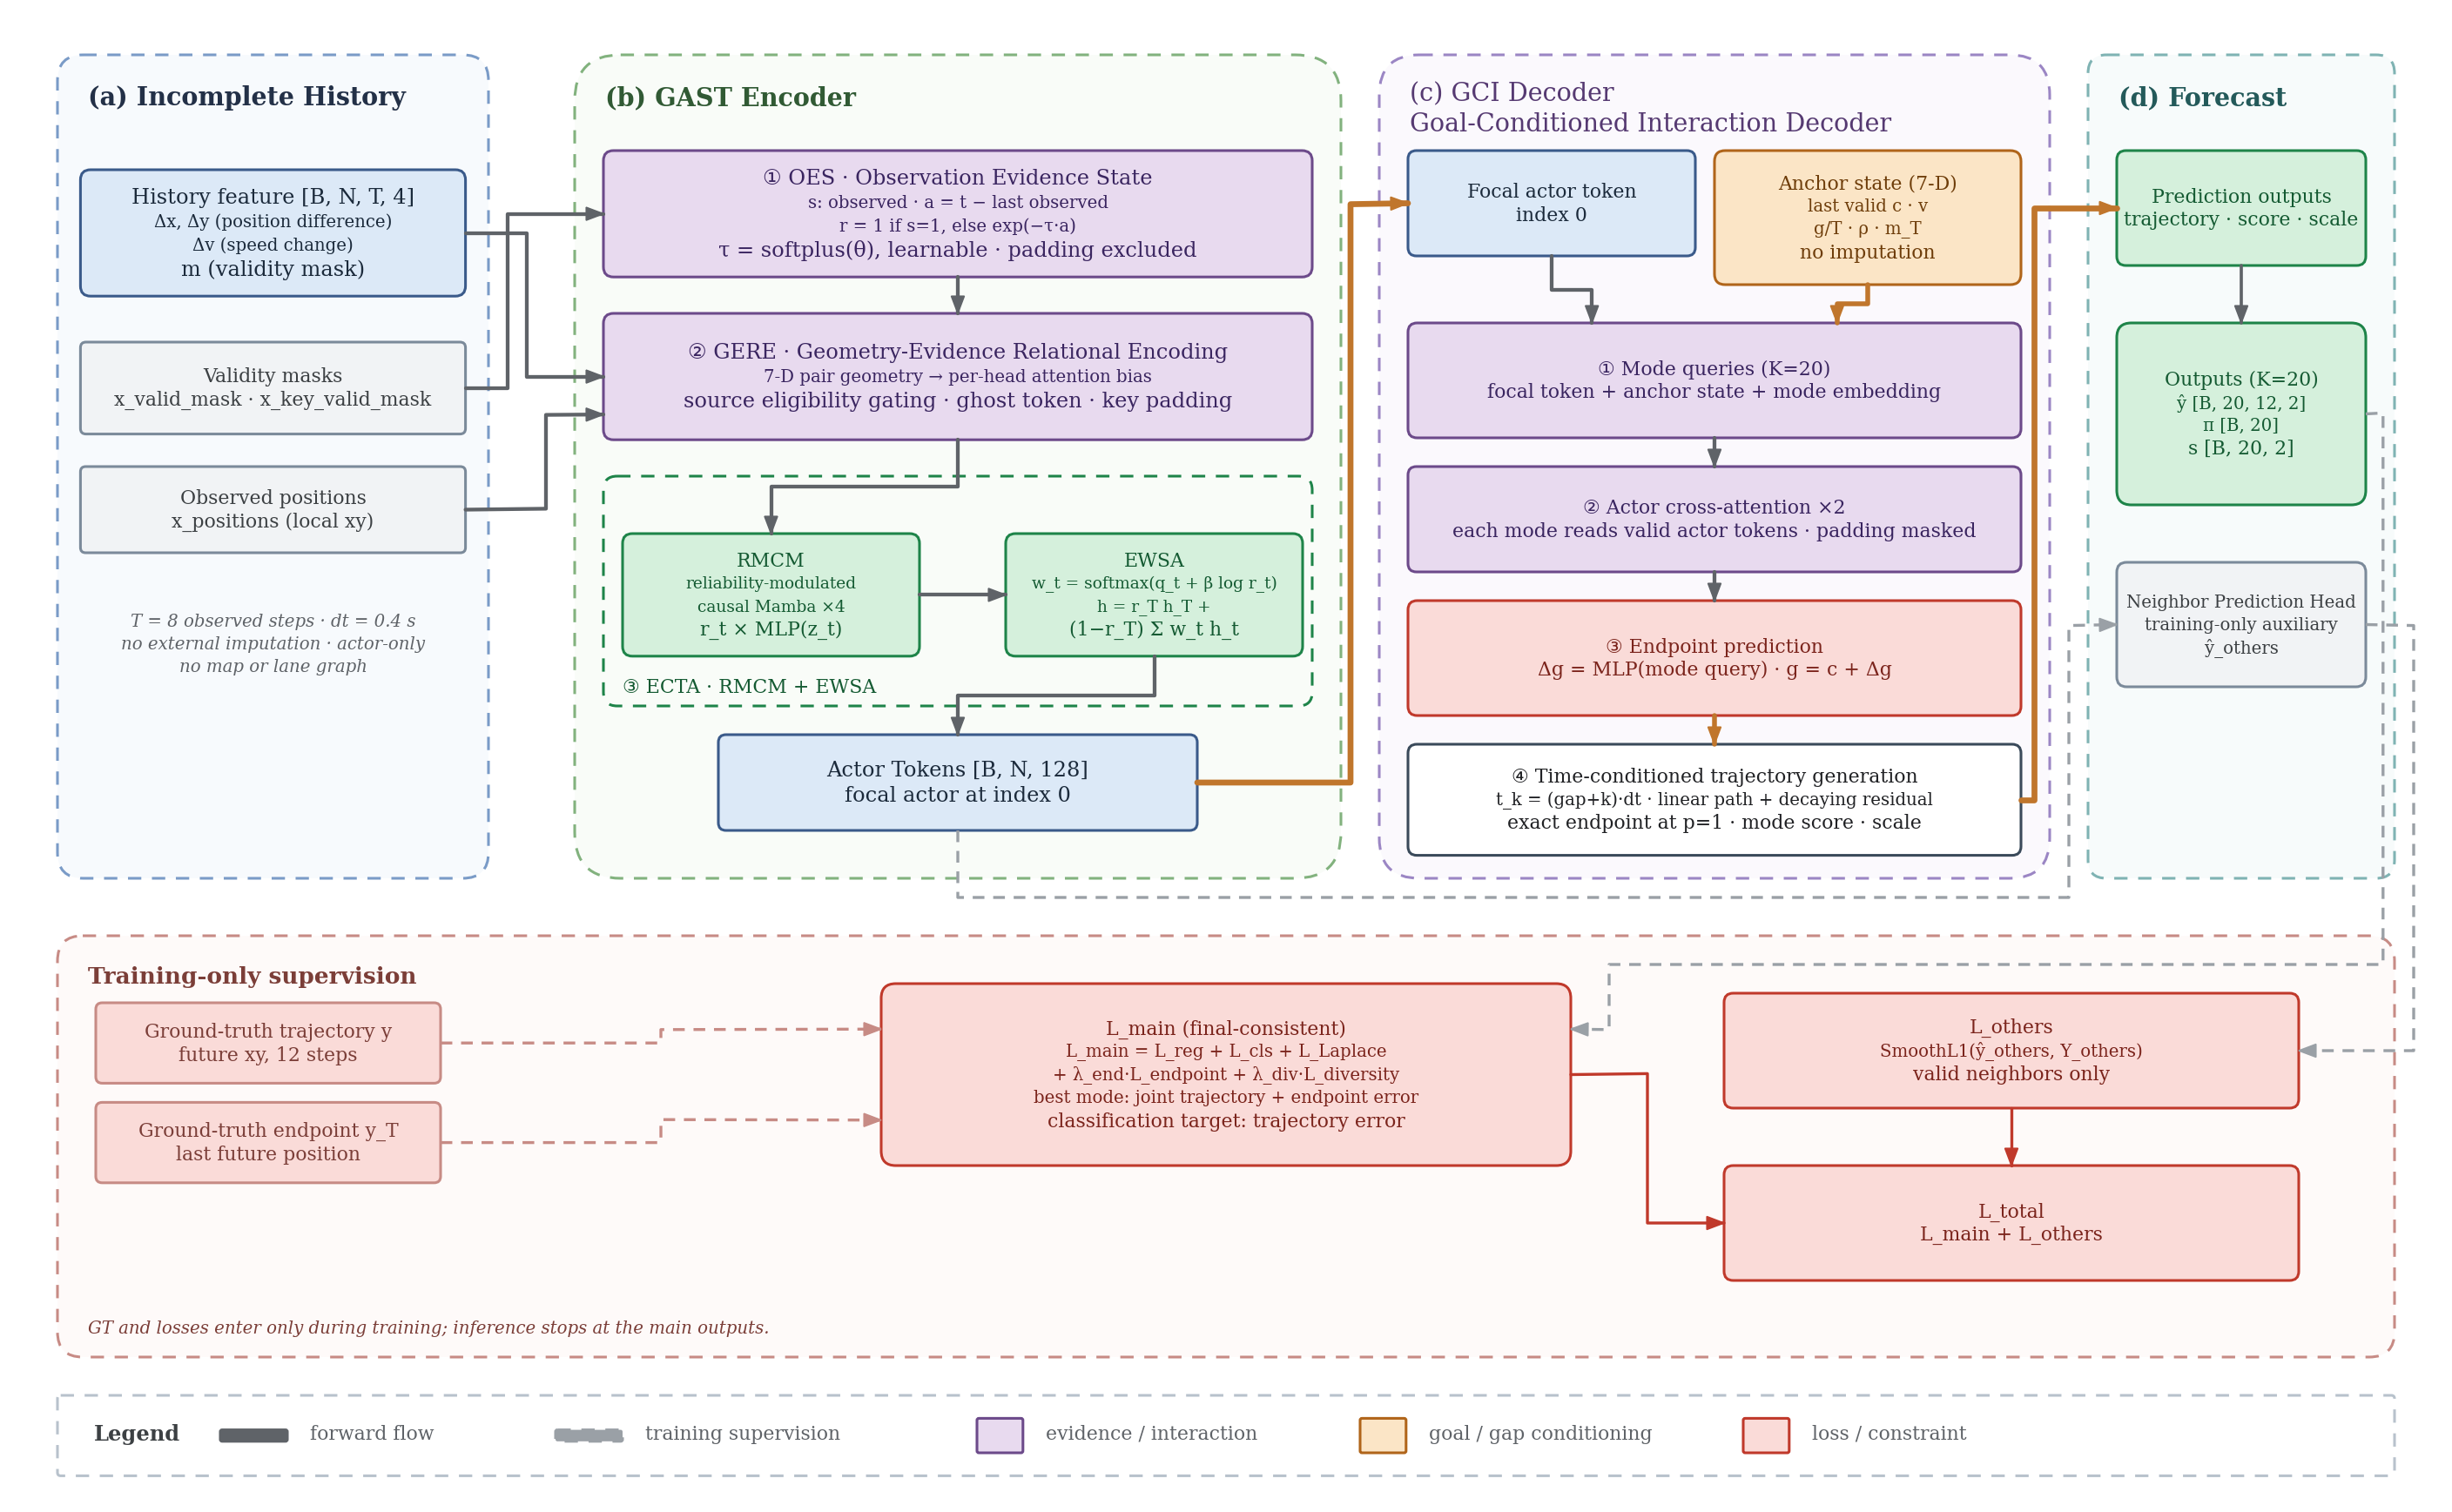
\includegraphics[width=0.94\textwidth]{figures/architecture_crop.png}
\caption{Architecture of GAST. (a)~The masked history is represented by positions, validity masks and observed positions only; missing entries are placeholders. (b)~The observation-evidence state (OES) drives GERE, which performs frame-wise relational attention with geometry bias and source eligibility, and ECTA, which scales the temporal input by evidence strength (RMCM) and aggregates states with an evidence-weighted readout (EWSA). (c)~The goal-conditioned decoder builds a seven-dimensional anchor state from the last observed frame, forms $K$ mode queries and predicts an endpoint plus a progress-conditioned residual per mode. (d)~Outputs are $K$ trajectories with probabilities and per-mode scales; the neighbour head is used only during training.}
\label{fig:arch}
\end{figure*}

\subsection{Observation-evidence state}
\label{sec:oes}

For pedestrian $i$ at history step $t$, let
\begin{equation}
a_{i,t}=t-\max\{t'\le t: m_{i,t'}=1\},
\label{eq:age}
\end{equation}
be the age of the most recent observation, with $a_{i,t}=t$ when no frame up to $t$ has been observed (a virtual observation is assumed immediately before the window). The state comprises three quantities: the eligibility $s_{i,t}=m_{i,t}$ that decides whether the frame may act as a source of evidence, the age $a_{i,t}$, and a reliability
\begin{equation}
r_{i,t}=m_{i,t}+(1-m_{i,t})\,\exp(-\tau\,a_{i,t}),\qquad \tau=\mathrm{softplus}(\vartheta),
\label{eq:reliability}
\end{equation}
with a single learnable scalar $\vartheta$ initialised so that $\tau\approx0.1$. Reliability is exactly one at observed frames and decays monotonically over a gap. Padded agents are excluded from the state, and $r$ is zero for them.

Two properties of \eqref{eq:reliability} matter. First, it is not a calibrated probability and we never interpret it as one: it is a task-internal reliability variable whose role is to order history states by evidential support. Second, it is an identity on fully observed histories ($r\equiv1$), so the evidence conditioning vanishes and GAST reduces to its backbone. This is what allows the model to be compared with complete-history architectures without a distribution shift.

\subsection{GERE: frame-wise relational encoding with geometry bias}
\label{sec:gere}

The per-frame input of agent $i$ is a four-dimensional vector
\begin{equation}
u_{i,t}=\big[\Delta p_{i,t},\ \Delta s_{i,t},\ m_{i,t}\big],
\label{eq:input}
\end{equation}
containing the position increment, the increment of the observed speed, and the validity flag, mapped by a patch embedding $h_{i,t}=\mathrm{PatchEmbed}(u_{i,t})$.

\textbf{Ghost token.} At each frame the model pools the validity pattern of the whole scene into a single token,
\begin{equation}
g_{t}=\mathrm{max}_{i\in\mathcal{V}_{t}}\ \psi\big(\mathbf{1}-m_{i,t}\big),
\label{eq:ghost}
\end{equation}
where $\psi$ is a two-layer embedding applied to the scalar mask broadcast over the channel dimension and $\mathcal{V}_{t}$ is the set of non-padded agents. The token is prepended to the $N$ agent tokens for that frame and removed after attention. Because its input is the mask and only the mask, it summarises \emph{who is currently observable} without carrying any positional content; it therefore cannot inject a phantom coordinate, but it does give every agent a shared description of the scene's current observability.

\textbf{Source eligibility.} Attention keys are restricted to the ghost token and to agents with $s_{j,t}=1$. All agents, including unobserved ones, remain valid queries. An unobserved agent can therefore read the current state of its neighbours and the scene summary, but its own stale feature is never attended to by others. This implements P2 and differs from simply adding the mask as a feature, which leaves a stale token in the key set.

\textbf{Geometry bias.} For every ordered pair $(i,j)$ the model computes a seven-dimensional relational descriptor from the observed geometry,
\begin{equation}
f_{ij,t}=\big[\Delta p_{ij},\ \log(1+\|\Delta p_{ij}\|),\ \Delta v_{ij},\ \cos\Delta\theta_{ij},\ \sin\Delta\theta_{ij}\big],
\label{eq:geom}
\end{equation}
where $\Delta p_{ij}=p_{j,t}-p_{i,t}$, $\Delta v_{ij}=v_{j,t}-v_{i,t}$ and $\Delta\theta_{ij}$ is the difference of heading angles. Velocities are estimated from the current observation and the previous \emph{observed} position, divided by the number of steps between them, so a gap does not create a spurious velocity spike; if either endpoint of the pair is unobserved, $f_{ij,t}=\mathbf{0}$. The descriptor is mapped to one bias per attention head,
\begin{equation}
B_{ij,t}^{(h)}=w_{2}^{(h)\top}\,\mathrm{GELU}\big(W_{1}f_{ij,t}\big),
\label{eq:bias}
\end{equation}
and added to the attention logits of the agent--agent block. The output projection of \eqref{eq:bias} is zero-initialised, so training starts from a geometry-agnostic relational encoder and the bias is learned only if it reduces the objective. The relational stage is applied per frame; its output is a sequence of spatial states for each agent.

\subsection{ECTA: evidence-conditioned causal temporal aggregation}
\label{sec:ecta}

\textbf{RMCM (reliability-modulated causal encoder).} The spatial states are projected and scaled by the reliability before entering a causal recurrence,
\begin{equation}
\tilde{x}_{i,t}=\mathrm{MLP}(x_{i,t})\cdot r_{i,t},
\qquad
u_{i,1:T}=\mathrm{SSM}_{\phi}(\tilde{x}_{i,1:T}),
\label{eq:rmcm}
\end{equation}
where $\mathrm{SSM}_{\phi}$ is a stack of four unidirectional selective state-space blocks \cite{gu2023mamba}. Causality is required because the forecast must not depend on future history positions, and it makes the encoder usable in streaming deployment. The modulation is a scalar per frame and channel-shared: it changes how strongly a state enters the recursion, not what the state represents. In particular, an observed frame enters with unit strength, whereas a frame that has been missing for three steps is attenuated by $e^{-3\tau}$ and is effectively prevented from overwriting the last reliable state with a decayed one.

\textbf{EWSA (evidence-weighted state aggregation).} Readout is not fixed to the last time step. With content scores $e_{i,t}=w^{\top}u_{i,t}$ and a temperature $\beta=1$, the model forms
\begin{equation}
\alpha_{i,t}=\mathrm{softmax}_{t}\big(e_{i,t}+\beta\log r_{i,t}\big),\qquad
\bar{h}_{i}=\sum_{t}\alpha_{i,t}\,u_{i,t},
\label{eq:ewsa}
\end{equation}
and gates the terminal state against this aggregate,
\begin{equation}
z_{i}=r_{i,T}\,u_{i,T}+\big(1-r_{i,T}\big)\bar{h}_{i}.
\label{eq:gate}
\end{equation}
When the last frame is observed, $z_{i}=u_{i,T}$ exactly and the readout is identical to a standard terminal readout. When it is missing, the model falls back to a weighted average of the available states, with the weights shaped both by learned content and by evidence strength. The gate is a hard switch in form but a soft one in value, since $r_{i,T}$ decays continuously with the terminal gap.

\subsection{Anchor-conditioned goal decoding}
\label{sec:decoder}

\textbf{Anchor state.} Let $\ell_{i}$ be the index of the last observed frame and $\ell'_{i}$ the index of the previous one. The decoder receives
\begin{equation}
\varphi_{i}=\Big[p_{i,\ell_i},\ v_{i},\ \tfrac{\delta_{i}}{T},\ \rho_{i},\ \mathbb{1}[\ell_{i}<T]\Big]\in\mathbb{R}^{7},
\label{eq:anchor}
\end{equation}
where $\delta_{i}=T-\ell_{i}+1$ is the number of steps from the last observation to the forecast origin, $v_{i}=(p_{i,\ell_i}-p_{i,\ell'_i})/(\ell_i-\ell'_i)$ is a gap-aware velocity (zero when only one frame is observed), $\rho_{i}=\frac{1}{T}\sum_{t}m_{i,t}$ is the observed fraction, and the last term marks terminal missingness. The anchor position is retained so that the module is defined in any coordinate frame; under the anchor-centred normalisation of Section~\ref{sec:task} it vanishes and the state is carried by the velocity and gap descriptors.

\textbf{Mode queries.} The pedestrian representation $z_{i}$ from \eqref{eq:gate} and the anchor embedding $e^{\varphi}_{i}=\mathrm{MLP}(\varphi_{i})$ are combined with a learned per-mode embedding $e_{k}$,
\begin{equation}
q_{i,k}=z_{i}+e^{\varphi}_{i}+e_{k},\qquad k=1,\dots,K,
\label{eq:query}
\end{equation}
and refined by two cross-attention layers over the scene's pedestrian tokens, with padded agents masked out. Each mode thus sees the context under its own anchor condition rather than sharing a single scene vector.

\textbf{Endpoint and trajectory.} A head maps each mode query to a displacement from the anchor,
\begin{equation}
\hat{y}_{i,k,H}=p_{i,\ell_i}+\Delta_{i,k},\qquad \Delta_{i,k}=\mathrm{MLP}(q_{i,k}).
\label{eq:endpoint}
\end{equation}
For step $t=1,\dots,H$, let $\tau_{t}=\delta_{i}+t-1$ be the elapsed steps between the anchor time and that future step, and let $p_{t}=\tau_{t}/(\delta_{i}+H-1)$ be the corresponding fraction of the anchor-to-endpoint interval. The trajectory is a straight skeleton plus a decaying residual,
\begin{equation}
\hat{y}_{i,k,t}=p_{i,\ell_i}+p_{t}\,\Delta_{i,k}+\big(1-p_{t}\big)\,g_{\psi}\big(q_{i,k},e(\Delta_{i,k}),e(\tau_{t}\Delta t)\big).
\label{eq:traj}
\end{equation}
The construction has three consequences. The first predicted point is already advanced along the skeleton by $\delta_{i}/(\delta_{i}+H-1)$, so a long terminal gap is not silently treated as if the pedestrian had waited at the last observed position. The residual has full freedom early in the horizon and vanishes exactly at $t=H$, so the endpoint of the output coincides with the predicted goal. And because $p_{t}$ is defined in units of the actual gap, the same module handles observed and terminal-missing samples without a special case.

\textbf{Mode probabilities and scales.} A scoring head reads the mode query, the endpoint embedding and the mean of the per-step queries, and produces logits whose softmax gives $\pi_{i,k}$. A parallel head outputs a per-step, per-axis Laplace scale $\sigma_{i,k,t}=\mathrm{ELU}(\cdot)+1.0001$, used by the likelihood term below; $\sigma$ is a dispersion parameter of the predicted distribution, not a calibrated confidence interval.

\subsection{Training objective}
\label{sec:loss}

Supervision is applied to the focal pedestrian (index 0 of each scene sample). For mode $k$ we compute the average displacement $d_{k}$ and the endpoint error $d^{\mathrm{end}}_{k}$ against the ground truth, and define the joint error $J_{k}=d_{k}+\lambda_{e}d^{\mathrm{end}}_{k}$ with $\lambda_{e}=1$. Two different modes are selected for two different purposes: the regression mode $k^{\ast}=\arg\min_{k}J_{k}$ balances shape and destination, while the classification target $k^{\dagger}=\arg\min_{k}d_{k}$ is defined by trajectory-level error alone. The loss is
\begin{equation}
\mathcal{L}=\mathcal{L}_{\mathrm{reg}}+\mathcal{L}_{\mathrm{cls}}
+\mathcal{L}_{\mathrm{NLL}}+\mathcal{L}_{\mathrm{end}}
+\lambda_{d}\mathcal{L}_{\mathrm{div}}+\mathcal{L}_{\mathrm{nbr}},
\label{eq:loss}
\end{equation}
where $\mathcal{L}_{\mathrm{reg}}=\mathrm{SmoothL1}(\hat{y}_{k^{\ast}},y)$, $\mathcal{L}_{\mathrm{cls}}=-\log\pi_{k^{\dagger}}$, $\mathcal{L}_{\mathrm{end}}=\mathrm{SmoothL1}(\hat{y}_{k^{\ast},H},y_{H})$, $\mathcal{L}_{\mathrm{nbr}}=\mathrm{SmoothL1}(\hat{y}^{\mathrm{nbr}},y^{\mathrm{nbr}})$, and $\mathcal{L}_{\mathrm{div}}=\mathbb{E}_{k\ne l}[0.5-\|\hat{y}_{k,H}-\hat{y}_{l,H}\|]_{+}$ is a hinge on pairwise endpoint distances; $\mathcal{L}_{\mathrm{NLL}}$ is the Laplace negative log-likelihood detailed in Appendix~\ref{app:loss}. The cross-entropy is evaluated with label smoothing $0.2$, the diversity weight is $\lambda_{d}=0.05$, and the margin is $0.5$~m. The likelihood term is computed on the trajectory-closest mode, $\log(2\sigma)+|y-\hat{y}|/\sigma$ averaged over steps and axes, combined with a soft-target cross-entropy $0.5\sum_{k}\tilde{\pi}_{k}\log\pi_{k}$ whose target $\tilde{\pi}$ is a temperature-softmax of the negative trajectory errors; it calibrates the dispersion and gently shapes the mode distribution without competing with the hard classification target. The neighbour term predicts the future of the other agents in the scene from their encoder states and is used only during training; at inference the model returns the $K$ candidate futures of the focal pedestrian and their probabilities.

The separation of $k^{\ast}$ and $k^{\dagger}$ is deliberate. Probability should rank modes by how well they explain the whole trajectory, whereas the endpoint head should be trained on the mode that best explains the destination. Sharing a single assignment forces one objective to compromise; separating them costs nothing at inference.

\subsection{Properties}

\textbf{Exact reduction.} With $m_{i,t}=1$ for all $t$, \eqref{eq:reliability} gives $r\equiv1$: \eqref{eq:rmcm} becomes a plain causal encoder, \eqref{eq:gate} returns the terminal state, and the anchor state carries only the observed velocity, with $\delta=1$, $\rho=1$ and no terminal flag. The gap-specific machinery therefore contributes nothing in this condition, and any difference from a complete-history baseline is attributable to the decoder and to the always-present scene-level token.

\textbf{No leakage.} Placeholders never enter a difference, a distance or a velocity: velocities are computed only between observed frames, pairwise geometry is zeroed when either endpoint is unobserved, and unobserved agents are removed from the key set. Ground-truth futures are used only in the loss.

\textbf{Cost.} The model has 1.19M parameters (0.60M encoder, 0.55M decoder), and inference is a single forward pass with $K=20$ parallel mode queries; no sampling loop is required. Per-frame relational attention is $O(N^{2})$ in the number of pedestrians in a frame, which is the same order as the social-attention baselines we compare against.

\section{Experiments}
\label{sec:exp}

\subsection{Experimental setup}
\label{sec:setup}

\textbf{Data and protocol.} All experiments use the TrajGap-Bench Mixed protocol of Section~\ref{sec:bench}: Mixed-train for fitting, Mixed-val for checkpoint selection on $\mathrm{minFDE}_{20}$ of the final head, Mixed-test evaluated once, five scenes, $T=8$, $H=12$, $K=20$. One model is trained per scene, following the release's per-scene splits. Every method is trained on the natural Mixed distribution; no method re-weights samples by missing count.

\textbf{Implementation.} GAST uses an embedding width of 128, 8 attention heads, four selective state-space blocks in the temporal stack, two cross-attention layers in the decoder, $K=20$ modes and dropout/drop-path 0.2. Training uses AdamW with learning rate $10^{-3}$, weight decay $10^{-4}$, 5 warm-up epochs, gradient clipping at norm 5, batch size 64 and bf16 mixed precision for at most 100 epochs; the selected checkpoints occur between epochs 33 and 58, so the budget is not binding. Each scene is trained on a single NVIDIA RTX 5880 Ada GPU. The model has 1.19M parameters. The seed is fixed to 2024 for all methods.

\textbf{Baselines.} We compare against six external baselines, spanning three families.
\begin{itemize}
\item \emph{Complete-history forecasters.} \textbf{SocialLSTM} \cite{alahi2016social} is run in a missing-aware variant (zero placeholder, LSTM state update skipped at missing frames, Gaussian-mixture head with $K=20$). \textbf{AgentFormer} \cite{yuan2021agentformer} receives an explicit per-frame validity channel and anchors the decoder at the last observed frame. \textbf{MoFlow} \cite{fu2025moflow} uses its official implementation with mask-aware features and a per-channel mean placeholder at missing steps. \textbf{Re} \cite{mao2025resonance} is run unmodified with zero-filled histories.
\item \emph{Imputation-aware forecaster.} \textbf{MS-TIP} \cite{chib2024mstip} couples a SAITS-based imputation branch with the predictor and is trained end-to-end; it represents the impute-and-predict family under the direct input constraint. \textbf{Social-STGCNN} \cite{mohamed2020social} is included as a graph-based reference; missing agents are represented as ghost nodes that neither send nor receive messages.
\end{itemize}
Methods without a mode-probability head (AgentFormer, Re, MS-TIP, Social-STGCNN) are excluded from the top-1 diagnostics but included in the primary metrics, which only require $K$ candidates. All methods see exactly the same test tensors.

\subsection{Main results}
\label{sec:main}

Table~\ref{tab:main} reports the primary comparison. GAST obtains the best macro average on both metrics, 0.3168/0.4831~m, and the best micro average, 0.2894/0.4716~m. Relative to the strongest external baseline (MoFlow), this is a reduction of 9.4\% in $\mathrm{minADE}_{20}$ and 7.6\% in $\mathrm{minFDE}_{20}$ on the macro average, and 7.5\%/5.3\% on the micro average. GAST is better than MoFlow on all five scenes for $\mathrm{minADE}_{20}$ and on four of five for $\mathrm{minFDE}_{20}$, the exception being ZARA1-M, where MoFlow is 1.8\% better.

The per-scene picture is more informative than the aggregate. GAST attains the best $\mathrm{minFDE}_{20}$ on ETH-M, UNIV-M and ZARA2-M, and the best $\mathrm{minADE}_{20}$ on ETH-M and UNIV-M. On HOTEL-M, AgentFormer is clearly better (0.2083/0.3316 against 0.2541/0.3769), and on ZARA1-M, MoFlow is better on $\mathrm{minFDE}_{20}$. The margin over the strongest external baseline is largest exactly on the scenes with the most heterogeneous motion (ETH-M: $-12.5\%$ on $\mathrm{minFDE}_{20}$ relative to MoFlow; UNIV-M: $-5.9\%$), and smallest on ZARA1-M ($+1.8\%$), a scene of slow, regular motion. We do not claim a uniform improvement, and Section~\ref{sec:disc} discusses what distinguishes the scenes on which the method helps.

The two weakest baselines are far behind. MS-TIP, the representative of imputation-aware joint training, is the second worst method, and Social-STGCNN, which represents unobserved agents as ghost nodes, is the worst. Both are trained under the same contract as every other method, so the gap is not a protocol artefact; it reflects the difficulty of the 8-frame setting, in which up to seven frames are absent and the gaps frequently reach the forecast origin. The classical social-pooling model is also well behind (0.4576/0.6079), which is expected given the short history and the absence of explicit multi-modality in its missing-aware variant.

\begin{table*}[t]
\centering
\footnotesize
\setlength{\tabcolsep}{3.2pt}
\caption{Main results on TrajGap-Bench Mixed-test ($K=20$, seed 2024). Cells are $\mathrm{minADE}_{20}$/$\mathrm{minFDE}_{20}$ in metres; lower is better. Macro is the unweighted mean over the five scenes; Micro is weighted by test-sample count. Best per scene and metric in bold. Methods marked $\dagger$ output unweighted samples and are excluded from top-1 diagnostics.}
\label{tab:main}
\begin{tabular}{@{}lccccccc@{}}
\toprule
Method & ETH-M & HOTEL-M & UNIV-M & ZARA1-M & ZARA2-M & Macro & Micro \\
\midrule
\textbf{GAST (ours)} & \textbf{0.5852}/\textbf{0.8212} & 0.2541/0.3769 & \textbf{0.3200}/\textbf{0.5244} & \textbf{0.2510}/0.4128 & 0.1738/\textbf{0.2801} & \textbf{0.3168}/\textbf{0.4831} & \textbf{0.2894}/\textbf{0.4716} \\
MoFlow & 0.6819/0.9389 & 0.2777/0.4247 & 0.3478/0.5572 & 0.2566/\textbf{0.4057} & 0.1839/0.2867 & 0.3496/0.5227 & 0.3129/0.4981 \\
AgentFormer & 0.7098/1.0436 & \textbf{0.2083}/\textbf{0.3316} & 0.4132/0.6796 & 0.3551/0.5795 & \textbf{0.1700}/0.4375 & 0.3911/0.6144 & 0.3795/0.6220 \\
SocialLSTM & 0.8430/1.0456 & 0.2924/0.3871 & 0.4543/0.6512 & 0.4126/0.5650 & 0.2858/0.3907 & 0.4576/0.6079 & 0.4193/0.5941 \\
Re$^{\dagger}$ & 0.9945/1.4262 & 0.7799/1.2808 & 0.5388/0.8408 & 0.4960/0.7470 & 0.3819/0.5928 & 0.6382/0.9775 & 0.5187/0.8085 \\
MS-TIP$^{\dagger}$ & 1.6345/2.0985 & 1.3102/1.5472 & 1.3240/1.1566 & 0.8842/1.1720 & 0.7663/0.9902 & 1.1838/1.3929 & 1.1991/1.1461 \\
Social-STGCNN$^{\dagger}$ & 2.1393/3.5048 & 1.3022/2.1624 & 0.9496/1.5336 & 1.4801/2.7038 & 0.8646/1.5258 & 1.3471/2.2861 & 0.9878/1.6409 \\
\bottomrule
\end{tabular}
\end{table*}

\subsection{Behaviour under increasing missingness}
\label{sec:severity}

Table~\ref{tab:severity} and Figure~\ref{fig:degrad} stratify the test set by the number of missing history frames. The benchmark's official sweep assigns equal test mass to each count from 0 to 7 (33{,}654 samples per bucket, with 67{,}308 for four because ETH-M contributes two four-frame buckets), which makes the buckets directly comparable.

The curves separate the methods in a way that the aggregate does not. GAST degrades most gracefully from zero to six missing frames: its $\mathrm{minFDE}_{20}$ rises by 19\% over that range, against +46\% for MoFlow and +65\% for SocialLSTM. The margin over the strongest external baseline widens monotonically with severity: GAST is 5.4\% better than MoFlow at zero missing frames, 6.6\% at three, 14.9\% at five and 22.6\% at six. This dose--response pattern is evidence that the improvement is produced by the evidence machinery rather than by extra capacity, since a capacity effect would not concentrate in the buckets where evidence is scarce.

At seven missing frames, only a single observation survives. All external baselines with mode sets collapse to 1.22--1.36~m and the ordering changes: MoFlow is best (1.2224), GAST second at 1.2731, SocialLSTM at 1.3587. With one frame there is no velocity, no heading and no gap structure to exploit, so the forecast is determined by the learned prior, and a method regularised for evidence routing has little left to route. We regard this as a boundary of the regime rather than a failure of the model, but it does mean that GAST should not be advertised as improving the single-frame case.

\begin{table*}[t]
\centering
\footnotesize
\setlength{\tabcolsep}{4.6pt}
\caption{Stratification by the number of missing history frames (macro average over five scenes, metres). Each bucket contains 33{,}654 test samples except four missing frames (67{,}308). Best value per bucket in bold.}
\label{tab:severity}
\begin{tabular}{@{}lcccccccc@{}}
\toprule
 & 0 & 1 & 2 & 3 & 4 & 5 & 6 & 7 \\
\midrule
\multicolumn{9}{@{}l}{\emph{$\mathrm{minADE}_{20}$}}\\
GAST & \textbf{0.2154} & \textbf{0.2192} & \textbf{0.2286} & \textbf{0.2336} & \textbf{0.2440} & \textbf{0.2629} & \textbf{0.2911} & 0.9126 \\
MoFlow & 0.2309 & 0.2390 & 0.2481 & 0.2706 & 0.2847 & 0.3221 & 0.3926 & \textbf{0.8734} \\
\midrule
\multicolumn{9}{@{}l}{\emph{$\mathrm{minFDE}_{20}$}}\\
GAST & \textbf{0.3590} & \textbf{0.3632} & \textbf{0.3756} & \textbf{0.3777} & \textbf{0.3854} & \textbf{0.4002} & \textbf{0.4281} & 1.2731 \\
MoFlow & 0.3793 & 0.3889 & 0.3968 & 0.4254 & 0.4341 & 0.4695 & 0.5534 & \textbf{1.2224} \\
\bottomrule
\end{tabular}
\end{table*}

\begin{figure*}[t]
\centering
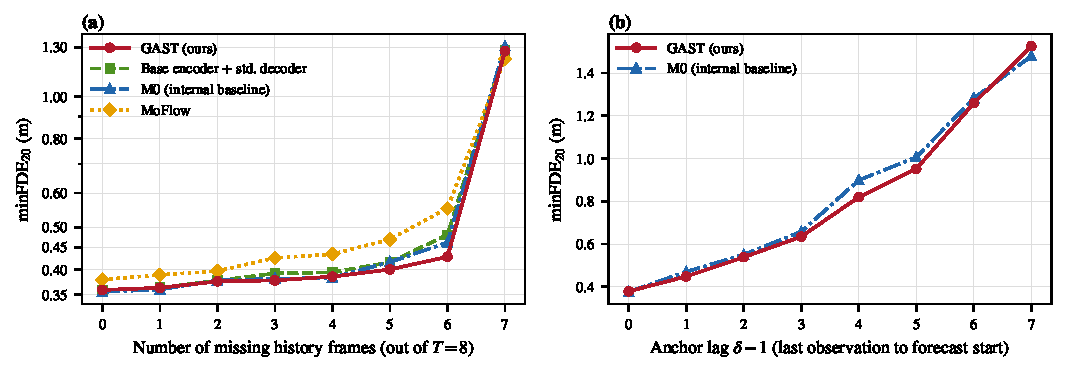
\includegraphics[width=\textwidth]{figures/degradation.pdf}
\caption{Degradation with respect to evidence loss (macro average over five scenes). (a)~$\mathrm{minFDE}_{20}$ as a function of the number of missing history frames, on a logarithmic scale; the dashed segment at seven frames reflects the qualitative change of regime in which a single observation remains. (b)~$\mathrm{minFDE}_{20}$ as a function of anchor lag, i.e.\ the number of steps between the last observation and the forecast origin. GAST's curve is flatter than the external baselines' at intermediate lags.}
\label{fig:degrad}
\end{figure*}

\subsection{Terminal missingness and anchor lag}
\label{sec:lag}

We report the same comparison along the two axes that the missing count confounds. Terminal missingness separates samples whose gap reaches the forecast origin from those whose gap ends earlier, and anchor lag counts the steps between the last observation and the origin. Among the external baselines, these diagnostics are available for SocialLSTM; MoFlow's evaluator emits only the missing-count axis.

The terminal group is the harder one for every method, and the gap between the groups is informative: relative to the non-terminal group, terminal-gap samples cost SocialLSTM $+75.0\%$ in $\mathrm{minFDE}_{20}$ (0.4547 to 0.7956), against $+61.4\%$ for GAST (0.3787 to 0.6112). GAST is 16.7\% better than SocialLSTM on the non-terminal group and 23.2\% better on the terminal group, so the relative advantage does not shrink where the anchor machinery is most exposed; this is the condition that the anchor state and the progress-conditioned skeleton were designed for.

Along anchor lag, GAST is better than SocialLSTM at every lag from 0 to 7, with the largest gaps at lags 3 and 4 ($-28.9\%$ and $-35.2\%$) and the smallest at the extreme lag 7 ($-7.4\%$), the regime in which only the first frame of the window is observed and the anchor is eight steps old. The shrinking margin at the extreme lag is the same phenomenon as the seven-missing bucket: beyond a certain evidence age, the estimate of the anchor velocity is dominated by noise, and a prior-driven forecast can approach an evidence-driven one. It suggests that the reliability decay should eventually saturate rather than continue to favour a very old state, which we leave to future work.

\subsection{Coverage versus ranking}
\label{sec:coverage}

Table~\ref{tab:top1} reports the top-1 diagnostics. GAST's $\mathrm{ADE@1}$/$\mathrm{FDE@1}$ are 0.9807/1.7887~m. Its $\mathrm{ADE@1}$ is statistically indistinguishable from MoFlow's (0.9814) and its $\mathrm{FDE@1}$ is 3.4\% worse than MoFlow's (1.7296), while its best-of-20 metrics are the best in the comparison and 7.6\% better than MoFlow's on the macro average. The dissociation between coverage and ranking is therefore mild relative to the strongest external baseline, but it is systematic: the top-1 margin narrows or reverses on scenes where the best-of-20 margin is large.

Our working hypothesis is that the goal-conditioned decoder, trained with an explicit diversity margin on endpoints and with trajectory-level mode labels, spreads the mode set and assigns probability mass more evenly, which improves coverage and simultaneously reduces the mass on the single best mode. This is a hypothesis about a mechanism, not a demonstrated causal explanation; we report it as an open problem, since a forecaster that is deployed behind a planner is usually consumed through its highest-probability mode.

\begin{table}[t]
\centering
\footnotesize
\setlength{\tabcolsep}{4.2pt}
\caption{Top-1 diagnostics (macro average, metres). $\mathrm{ADE@1}$/$\mathrm{FDE@1}$ use the highest-probability mode. Methods without mode probabilities are omitted.}
\label{tab:top1}
\begin{tabular}{@{}lcc@{}}
\toprule
Method & $\mathrm{ADE@1}$ & $\mathrm{FDE@1}$ \\
\midrule
MoFlow & \textbf{0.9814} & \textbf{1.7296} \\
GAST & 0.9807 & 1.7887 \\
SocialLSTM & 1.3278 & 2.1865 \\
\bottomrule
\end{tabular}
\end{table}

\subsection{Reproducibility}
\label{sec:repro}

The protocol, the Mixed adapter, the training runner, the evaluator and the model configuration are released as a single repository. Every run writes a manifest containing the git revision, the resolved configuration, the data files consumed, the checkpoint rule and the environment (Python, PyTorch and CUDA versions). Evaluation emits a JSON file with per-sample diagnostics for each of the five stratification axes, from which all tables in this paper are generated by script rather than transcribed by hand. The Laplace likelihood has two numerically equivalent implementations, one of which is vectorised; an equivalence gate verifies that their gradients agree to machine precision, and the implementation used by each run is recorded in its manifest.

\section{Discussion}
\label{sec:disc}

\subsection{What the evidence state buys, and where}
The stratified results support a specific reading of the method. GAST does not improve forecasting by being a larger or better-tuned model; its advantage is concentrated exactly where the observation record is degraded, and it vanishes or reverses where the record is complete or nearly absent. Three facts form this argument. The relative gain over M0 grows with severity across the high-missing range ($-3.9\%$ at five missing frames and $-7.3\%$ at six, against $+1.0\%$ when nothing is missing). The terminal-missing group, which is the condition that the anchor machinery targets, shows a 3.6\% reduction while the non-terminal group does not. And the anchor-lag curve is flatter than M0's over lags one to six. The gain is not strictly monotone in the missing count---the middle buckets fluctuate within a percentage point---but its concentration in the buckets where evidence is scarce is what a capacity explanation does not predict.

The reversal at lag seven is equally informative. When the anchor is eight frames old, the gap-aware velocity is estimated from a single surviving observation pair and is dominated by noise, while the reliability gate still prefers that stale state over the aggregate. A model that instead leans on a learned motion prior can be more accurate. This suggests that the evidence weighting should saturate: beyond some age, the reliability of a state should be constant rather than continuing to decay, and the decoder should be allowed to trust the prior. We did not tune this boundary on test data, and we report it as a limitation of the current formulation rather than as a hyperparameter choice.

\subsection{Scene heterogeneity}
The per-scene results are not uniform: GAST is the best method on ETH-M, UNIV-M and ZARA2-M, is behind M0 on ZARA1-M and HOTEL-M, and is behind AgentFormer on HOTEL-M by a wide margin. We can offer a hypothesis, although the benchmark does not permit a clean test of it. HOTEL-M and ZARA1-M are scenes with relatively slow, regular motion and strong scene constraints, where a unimodal extrapolation from the last observation is already accurate; the endpoint-conditioned decoder, which is designed to place probability mass on distinct destinations, adds variance without adding accuracy. ETH-M and UNIV-M contain more heterogeneous motion and more frequent direction changes, where the destination is genuinely uncertain and an explicit endpoint hypothesis helps. If this reading is correct, the decoder should be conditioned on a scene- or sample-level estimate of endpoint uncertainty rather than applied uniformly. We regard this as the most promising direction for closing the scene-level gap, but the present evidence is correlational.

\subsection{Coverage and ranking}
The dissociation between best-of-20 coverage and top-1 ranking is the most consequential negative result in this study. GAST improves the metrics that the benchmark ranks by, and degrades the metric that a downstream planner most often consumes, by roughly 11--13\%. Since the encoder-only variants do not show the degradation, the decoder is the plausible locus, and the diversity term plus the trajectory-level classification target are the plausible mechanisms. A direct test would be to retrain with the diversity weight annealed to zero and with a joint classification target, and to measure both metric families; we did not run this ablation, and we therefore state the diagnosis as a hypothesis. Until it is resolved, GAST should be used where best-of-$K$ coverage matters, and its top-1 mode should not be treated as a calibrated intention estimate.

\subsection{Limitations}
\textbf{Single seed.} All numbers are from one seed per scene. We have no confidence intervals, and we observed a 4.4\% run-to-run difference on UNIV-M between two runs of the same configuration during development. Differences of a few percent on a single scene, such as the 1.7\% macro margin over M0, are therefore within the range that a second seed could plausibly move. The macro ordering against the external baselines is far outside that range, but the ordering among the internal variants is not. A multi-seed study with paired, trajectory-clustered bootstrap is required before any claim of a stable improvement over M0.

\textbf{Protocol dependence.} TrajGap-Bench is a controlled stress test built on synthetic masks. Its missingness distribution is not claimed to match any real tracker, and the benchmark is restricted to five ETH/UCY scenes with an 8-frame history. External validity on real perception output and on other datasets (e.g.\ SDD or Argoverse) is untested.

\textbf{Test-set dependence.} The test split contains the same latent trajectory under multiple masks. Our aggregations treat samples as independent, which overstates the effective sample size for any significance statement. The released per-sample diagnostics include the source track identifier precisely so that clustered inference can be performed later.

\textbf{Ablation granularity.} As discussed in Section~\ref{sec:ablation}, the build-up sequence changes encoder and decoder together, so the contributions of GERE, ECTA and the goal decoder are not separated. The UT-ENC arm was also produced under the earlier checkpoint monitor.

\textbf{Missing comparisons.} We do not report a two-stage imputation baseline inside the direct table, because the setting exposes the model to more information and must be reported separately; the comparison is therefore absent rather than negative. We also do not report inference latency, which matters for deployment.

\subsection{Implications for benchmark design}
Two design choices in the protocol proved to be load-bearing. Merging Easy and Hard into a single Mixed split prevents a model from being selected on the difficulty at which it happens to be strongest, and it makes the missing-count stratification a diagnostic rather than a leaderboard. Fixing the checkpoint to the final head's validation $\mathrm{minFDE}_{20}$ removes a degree of freedom that otherwise silently differs across papers. Both choices are cheap to adopt and, in our experience, change conclusions: several variants that looked better under a per-difficulty protocol did not survive the Mixed contract. We recommend that future work on missing-history forecasting report at least the missing-count and terminal-missingness stratifications, since the aggregate can hide a reversal of the kind documented at seven missing frames.

\section{Conclusion}
\label{sec:concl}

We have argued that incomplete histories should be treated as a prediction condition rather than as data to be repaired, and we have supported the argument with a protocol and a model. TrajGap-Bench freezes a single Mixed contract on the public TrajImpute release---one split construction, one checkpoint rule, two metrics, five diagnostic stratifications---so that methods which consume incomplete histories can be compared on identical terms. GAST carries an observation-evidence state through frame-wise relational attention, a reliability-modulated causal state-space encoder and an anchor-conditioned goal decoder, and it never imputes a coordinate.

On 302{,}886 test samples from five scenes, GAST obtains the best macro-averaged best-of-20 error among the compared methods (0.3168/0.4831~m), 9.4\%/7.6\% below the strongest external baseline. Its advantage over the strongest internal baseline is small in aggregate (1.7\%/1.8\%) but structured: it grows monotonically with missing-frame count up to six frames, is largest on terminal gaps, and reverses when a single observation survives. We have also reported two results that qualify the contribution: the improvement is not uniform across scenes, and it is accompanied by an 11--13\% degradation of top-1 ranking, which we trace to the decoder and leave as an open problem.

The next steps follow directly from the limitations. A multi-seed study with trajectory-clustered statistics is needed to establish whether the margin over M0 is stable. A four-arm ablation should separate the encoder and decoder contributions. A saturation rule for evidence age should address the reversal at the oldest anchor. And the same protocol should be extended to other observation geometries and to trajectories produced by a real perception stack, where the missingness distribution is not synthetic.


\appendix
\section{Objective and Implementation Details}
\label{app:impl}

\subsection{Explicit form of the auxiliary terms}
\label{app:loss}

Let $y\in\mathbb{R}^{H\times2}$ be the future of the focal pedestrian, $\hat{y}_{k}$ the $k$-th candidate and $\pi\in\Delta^{K-1}$ the mode distribution. With per-step errors $e_{k,t}=\|\hat{y}_{k,t}-y_{t}\|$, $d_{k}=\frac{1}{H}\sum_{t}e_{k,t}$ and $d^{\mathrm{end}}_{k}=\|\hat{y}_{k,H}-y_{H}\|$, the terms of \eqref{eq:loss} that are not written out in the main text are
\begin{equation}
\begin{aligned}
\mathcal{L}_{\mathrm{NLL}}=\ &\frac{1}{2H}\sum_{t,c}\Big[\log\big(2\sigma_{k^{\ast},t,c}\big)+\frac{|y_{t,c}-\hat{y}_{k^{\ast},t,c}|}{\sigma_{k^{\ast},t,c}}\Big]\\
&-\frac{1}{2}\sum_{k}\tilde{\pi}_{k}\log\pi_{k},
\end{aligned}
\label{eq:nll}
\end{equation}
with the soft target
\begin{equation}
\tilde{\pi}_{k}=\mathrm{softmax}_{k}\big(-d_{k}/H\big),\qquad
k^{\ast}=\arg\min_{k}\big(d_{k}+\lambda_{e}d^{\mathrm{end}}_{k}\big),
\label{eq:softtarget}
\end{equation}
$\lambda_{e}=1$, and $k^{\dagger}=\arg\min_{k}d_{k}$. The soft target is detached from the graph. The classification term $\mathcal{L}_{\mathrm{cls}}=-\log\pi_{k^{\dagger}}$ uses label smoothing $0.2$; the diversity term uses $\lambda_{d}=0.05$ and a margin of $0.5$~m. The neighbour term is a SmoothL1 loss over the futures of all non-padded agents other than the focal one, computed from a two-layer head applied to their encoder states, and it is active only during training.

\subsection{Per-scene stratification}
\label{app:strat}

Table~\ref{tab:appstrat} reports $\mathrm{minFDE}_{20}$ for GAST on each scene and each missing-frame count. The scene-level shape mirrors the macro curve: ETH-M and HOTEL-M are the least sensitive scenes up to six missing frames, UNIV-M and ZARA1-M degrade more steadily, and every scene exhibits the discontinuity at seven missing frames. HOTEL-M is the extreme case, with a nearly flat curve from zero to six missing frames (0.1835 to 0.1957~m) followed by a jump to 1.9085~m; this is consistent with the low-speed, highly constrained motion in that scene, where a single observation still constrains the destination well.

\begin{table}[t]
\centering
\scriptsize
\setlength{\tabcolsep}{2.6pt}
\caption{GAST per-scene $\mathrm{minFDE}_{20}$ (m) by number of missing history frames. ETH-M has 362 samples in the four-frame bucket and 181 in each other bucket; all other scenes have 181 per bucket.}
\label{tab:appstrat}
\begin{tabular}{@{}lcccccccc@{}}
\toprule
Scene & 0 & 1 & 2 & 3 & 4 & 5 & 6 & 7 \\
\midrule
ETH-M   & 0.6641 & 0.6755 & 0.7196 & 0.7001 & 0.6988 & 0.7026 & 0.7314 & 1.7995 \\
HOTEL-M & 0.1835 & 0.1841 & 0.1806 & 0.1841 & 0.1847 & 0.1865 & 0.1957 & 1.9085 \\
UNIV-M  & 0.3997 & 0.4068 & 0.4176 & 0.4270 & 0.4427 & 0.4688 & 0.5048 & 1.2093 \\
ZARA1-M & 0.3199 & 0.3214 & 0.3292 & 0.3392 & 0.3523 & 0.3812 & 0.4185 & 0.9013 \\
ZARA2-M & 0.2276 & 0.2281 & 0.2312 & 0.2379 & 0.2483 & 0.2621 & 0.2902 & 0.5469 \\
\bottomrule
\end{tabular}
\end{table}

\subsection{Hyperparameters and compute}
\label{app:hparams}

\begin{table}[t]
\centering
\footnotesize
\caption{Training configuration shared by all GAST runs.}
\label{tab:hparams}
\begin{tabular}{@{}ll@{}}
\toprule
Item & Value \\
\midrule
History / horizon & 8 / 12 frames, $\Delta t=0.4$~s \\
Embedding width & 128 \\
Attention heads & 8 \\
Temporal stack depth & 4 (unidirectional SSM) \\
Decoder cross-attention & 2 layers \\
Modes $K$ & 20 \\
Dropout / drop-path & 0.2 / 0.2 \\
Optimiser & AdamW, lr $10^{-3}$, wd $10^{-4}$ \\
Schedule & 5 warm-up epochs, 100 epochs max \\
Batch size / precision & 64 / bf16 \\
Gradient clipping & norm 5 \\
Parameters & 1.19M (0.60M encoder, 0.55M decoder) \\
Checkpoint monitor & Mixed-val $\mathrm{minFDE}_{20}$, final head \\
Selected epochs & 58 / 41 / 42 / 33 / 49 \\
Hardware & 1$\times$ RTX 5880 Ada per scene \\
Seed & 2024 \\
\bottomrule
\end{tabular}
\end{table}

The selected epochs are listed in scene order (ETH-M, HOTEL-M, UNIV-M, ZARA1-M, ZARA2-M). No run reached the 100-epoch budget, so the reported results are not truncation-limited. The reliability temperature is parameterised as $\tau=\mathrm{softplus}(\vartheta)$ with $\vartheta$ initialised at $-2.252$, which gives $\tau\approx0.10$ and a half-life of roughly seven frames at initialisation; the parameter is learned jointly with the rest of the model.

\subsection{Reproducibility checklist}
\label{app:checklist}

\begin{itemize}
\item \textbf{Data.} Public TrajImpute release; the exact files consumed by each run are recorded in its manifest. No data beyond the release is used.
\item \textbf{Splits.} Mixed train/val/test as defined in Section~\ref{sec:mixed}; the test split is never used for model selection.
\item \textbf{Seeds.} One seed (2024) per scene for all methods; the limitation is stated in Section~\ref{sec:disc}.
\item \textbf{Metrics.} $\mathrm{minADE}_{20}$ and $\mathrm{minFDE}_{20}$ computed by a single evaluator for all methods; top-1 metrics reported only where mode probabilities exist.
\item \textbf{Artefacts.} Each run emits a manifest (git revision, resolved config, environment) and an evaluation JSON with per-sample diagnostics; all tables in the paper are generated from these files by script.
\item \textbf{Code.} The Mixed adapter, training runner, evaluator and model definition are released with the paper.
\end{itemize}


\begin{thebibliography}{99}
\footnotesize

\bibitem{alahi2016social}
A.~Alahi, K.~Goel, V.~Ramanathan, A.~Robicquet, L.~Fei-Fei, and S.~Savarese, ``Social LSTM: Human trajectory prediction in crowded spaces,'' in \emph{Proc. IEEE Conf. Computer Vision and Pattern Recognition (CVPR)}, 2016, pp. 961--971.

\bibitem{gupta2018social}
A.~Gupta, J.~Johnson, L.~Fei-Fei, S.~Savarese, and A.~Alahi, ``Social GAN: Socially acceptable trajectories with generative adversarial networks,'' in \emph{Proc. IEEE Conf. Computer Vision and Pattern Recognition (CVPR)}, 2018, pp. 2255--2264.

\bibitem{mohamed2020social}
A.~Mohamed, K.~Qian, M.~Elhoseiny, and C.~Claudel, ``Social-STGCNN: A social spatio-temporal graph convolutional neural network for human trajectory prediction,'' in \emph{Proc. IEEE/CVF Conf. Computer Vision and Pattern Recognition (CVPR)}, 2020, pp. 14424--14432.

\bibitem{yuan2021agentformer}
Y.~Yuan, X.~Weng, Y.~Ou, and K.~M.~Kitani, ``AgentFormer: Agent-aware transformers for socio-temporal multi-agent forecasting,'' in \emph{Proc. IEEE/CVF Int. Conf. Computer Vision (ICCV)}, 2021, pp. 9793--9803.

\bibitem{liang2020lane}
M.~Liang, B.~Yang, R.~Hu, Y.~Chen, R.~Liao, S.~Feng, and R.~Urtasun, ``Learning lane graph representations for motion forecasting,'' in \emph{Proc. European Conf. Computer Vision (ECCV)}, 2020, pp. 541--556.

\bibitem{gao2020vectornet}
J.~Gao, C.~Sun, H.~Zhao, Y.~Shen, D.~Anguelov, C.~Li, and C.~Schmid, ``VectorNet: Encoding HD maps and agent dynamics from vectorized representation,'' in \emph{Proc. IEEE/CVF Conf. Computer Vision and Pattern Recognition (CVPR)}, 2020, pp. 11525--11533.

\bibitem{mangalam2020not}
K.~Mangalam, H.~Girase, S.~Agarwal, K.~H.~Lee, S.~Li, and D.~Melni\v{c}uk, ``It is not the journey but the destination: Endpoint conditioned trajectory prediction,'' in \emph{Proc. European Conf. Computer Vision (ECCV)}, 2020, pp. 759--776.

\bibitem{salzmann2020trajectron}
T.~Salzmann, B.~Ivanovic, P.~Chakravarty, and M.~Pavone, ``Trajectron++: Dynamically-feasible trajectory forecasting with heterogeneous data,'' in \emph{Proc. European Conf. Computer Vision (ECCV)}, 2020, pp. 683--700.

\bibitem{fu2025moflow}
Y.~Fu, Q.~Yan, K.~Li, L.~Liao, and W.~Wang, ``MoFlow: One-step flow matching for human trajectory forecasting via implicit maximum likelihood estimation based distillation,'' in \emph{Proc. IEEE/CVF Conf. Computer Vision and Pattern Recognition (CVPR)}, 2025, pp. 17282--17293.

\bibitem{zhang2024demo}
B.~Zhang, N.~Song, and L.~Zhang, ``DeMo: Decoupling motion forecasting into directional intentions and dynamic states,'' in \emph{Advances in Neural Information Processing Systems (NeurIPS)}, vol.~37, 2024, pp. 106582--106606.

\bibitem{chib2024pedestrian}
P.~S.~Chib and P.~Singh, ``Pedestrian trajectory prediction with missing data: Datasets, imputation, and benchmarking,'' in \emph{Advances in Neural Information Processing Systems (NeurIPS), Datasets and Benchmarks Track}, 2024.

\bibitem{xu2023uncovering}
Y.~Xu, A.~Bazarjani, H.-G.~Chi, C.~Huang, and S.-C.~Huang, ``Uncovering the missing pattern: Unified framework towards trajectory imputation and prediction,'' in \emph{Proc. IEEE/CVF Conf. Computer Vision and Pattern Recognition (CVPR)}, 2023, pp. 9632--9643.

\bibitem{chib2024mstip}
P.~S.~Chib, A.~Nath, P.~Kabra, and P.~Singh, ``MS-TIP: Imputation aware pedestrian trajectory prediction,'' in \emph{Proc. Int. Conf. Machine Learning (ICML)}, PMLR, vol. 235, 2024, pp. 8389--8402.

\bibitem{chib2026hypergraph}
P.~S.~Chib and P.~Singh, ``Multi-scale hypergraphs for trajectory imputation and prediction in real-world scenarios,'' \emph{Expert Systems with Applications}, vol.~296, p. 129156, 2026.

\bibitem{sun2025rmpyolo}
J.~Sun, J.~Li, T.~Liu, et al., ``RMP-YOLO: A robust motion predictor for partially observable scenarios even if you only look once,'' in \emph{Proc. IEEE Int. Conf. Robotics and Automation (ICRA)}, 2025, pp. 1024--1031.

\bibitem{chen2023trajmae}
H.~Chen, J.~Wang, K.~Shao, and S.~Liu, ``Traj-MAE: Masked autoencoders for trajectory prediction,'' in \emph{Proc. IEEE/CVF Int. Conf. Computer Vision (ICCV)}, 2023, pp. 8317--8328.

\bibitem{yang2023rmp}
Y.~Yang, Q.~Zhang, T.~Gilles, N.~Batool, and M.~Folgheraiter, ``RMP: A random mask pretrain framework for motion prediction,'' in \emph{Proc. IEEE Int. Conf. Intelligent Transportation Systems (ITSC)}, 2023, pp. 3717--3723.

\bibitem{chib2023dropping}
P.~S.~Chib and P.~Singh, ``Improving trajectory prediction in dynamic multi-agent environment by dropping waypoints,'' \emph{arXiv:2309.17338}, 2023.

\bibitem{sun2022momentary}
J.~Sun, Y.~Li, L.~Chai, H.~Fang, Y.~Xu, and L.~Zheng, ``Human trajectory prediction with momentary observation,'' in \emph{Proc. IEEE/CVF Conf. Computer Vision and Pattern Recognition (CVPR)}, 2022, pp. 6457--6466.

\bibitem{monti2022howmany}
A.~Monti, A.~Porrello, S.~Calderara, and R.~Cucchiara, ``How many observations are enough? Knowledge distillation for trajectory forecasting,'' in \emph{Proc. IEEE/CVF Conf. Computer Vision and Pattern Recognition (CVPR)}, 2022, pp. 6553--6562.

\bibitem{qiu2025adapting}
R.~Qiu, J.~Gong, X.~Zhang, et al., ``Adapting to observation length of trajectory prediction via contrastive learning,'' in \emph{Proc. IEEE/CVF Conf. Computer Vision and Pattern Recognition (CVPR)}, 2025, pp. 1645--1654.

\bibitem{kosaraju2020social}
V.~Kosaraju, A.~Sadeghian, R.~Mart\'in-Mart\'in, I.~Reid, H.~Rezatofighi, and S.~Savarese, ``Social-BiGAT: Multimodal trajectory forecasting using Bicycle-GAN and graph attention networks,'' in \emph{Proc. Int. Conf. Learning Representations (ICLR)}, 2020.

\bibitem{ngiam2022scene}
J.~Ngiam, B.~Caine, V.~Vasudevan, Z.~Zhang, H.-T.~L.~Chiang, J.~Ling, R.~Roelofs, A.~Bewley, C.~Liu, A.~Venugopal, S.~Vaswani, and D.~Anguelov, ``Scene Transformer: A unified architecture for predicting future trajectories of multiple agents,'' in \emph{Proc. Int. Conf. Learning Representations (ICLR)}, 2022.

\bibitem{shi2022motion}
S.~Shi, L.~Jiang, D.~Dai, and B.~Schiele, ``Motion Transformer with global intention localization and local movement refinement,'' in \emph{Advances in Neural Information Processing Systems (NeurIPS)}, 2022.

\bibitem{nayakanti2022wayformer}
N.~Nayakanti, S.~Al-Rfou, K.~Zhou, J.~Go, K.~Wee, and D.~Krueger, ``Wayformer: Motion forecasting via simple and efficient attention networks,'' in \emph{Proc. Conf. Robot Learning (CoRL)}, 2022.

\bibitem{little2019missing}
R.~J.~A.~Little and D.~B.~Rubin, \emph{Statistical Analysis with Missing Data}, 3rd ed. Hoboken, NJ: Wiley, 2019.

\bibitem{vanbuuren2018flexible}
S.~van~Buuren, \emph{Flexible Imputation of Missing Data}, 2nd ed. Boca Raton, FL: CRC Press, 2018.

\bibitem{yoon2018gain}
J.~Yoon, J.~Jordon, and M.~van~der~Schaar, ``GAIN: Missing data imputation using generative adversarial nets,'' in \emph{Proc. Int. Conf. Machine Learning (ICML)}, 2018, pp. 5689--5698.

\bibitem{cao2018brits}
W.~Cao, D.~Wang, J.~Li, H.~Zhou, L.~Li, and Y.~Li, ``BRITS: Bidirectional recurrent imputation for time series,'' in \emph{Advances in Neural Information Processing Systems (NeurIPS)}, 2018, pp. 6775--6785.

\bibitem{che2018gru}
Z.~Che, S.~Puri, K.~Cho, D.~Levy, and S.~Ermon, ``Recurrent neural networks for multivariate time series with missing values,'' \emph{Scientific Reports}, vol.~8, no.~1, p. 6085, 2018.

\bibitem{du2023saits}
W.~Du, D.~C\^ot\'e, and Y.~Liu, ``SAITS: Self-attention-based imputation for time series,'' \emph{Expert Systems with Applications}, vol.~219, 2023.

\bibitem{hossain2025beyond}
Z.~T.~Hossain and M.~Milani, ``Beyond accuracy: An empirical study of uncertainty estimation in imputation,'' \emph{arXiv:2511.21607}, 2025.

\bibitem{itkina2022interpretable}
M.~Itkina and M.~J.~Kochenderfer, ``Interpretable self-aware neural networks for robust trajectory prediction,'' in \emph{Proc. Conf. Robot Learning (CoRL)}, PMLR, vol. 205, 2022, pp. 606--617.

\bibitem{nayak2023deepensembles}
A.~Nayak, A.~Eskandarian, and Z.~Doerzaph, ``Pedestrian trajectory forecasting using deep ensembles under sensing uncertainty,'' \emph{arXiv:2305.16620}, 2023.

\bibitem{wei2024navigation}
R.~Wei, J.~Lee, S.~Wakayama, and M.~S.~Ryu, ``Navigation under uncertainty: Trajectory prediction and occlusion reasoning with switching dynamical systems,'' \emph{arXiv:2410.10653}, 2024.

\bibitem{mohta2021multisensor}
A.~Mohta, F.-C.~Chou, B.~C.~Becker, S.~N.~Srinivasa, and S.~Scherer, ``Investigating the effect of sensor modalities in multi-sensor detection-prediction models,'' \emph{arXiv:2101.03279}, 2021.

\bibitem{sanchez2023robustness}
M.~Mu\~noz~S\'anchez, E.~Silvas, J.~Elfring, and M.~Zgonc, ``Robustness benchmark of road user trajectory prediction models for automated driving,'' \emph{IFAC-PapersOnLine}, vol.~56, no.~2, pp. 4865--4870, 2023.

\bibitem{sinopoli2004kalman}
B.~Sinopoli, L.~Schenato, M.~Franceschetti, K.~Poolla, M.~I.~Jordan, and S.~S.~Sastry, ``Kalman filtering with intermittent observations,'' \emph{IEEE Trans. Automatic Control}, vol.~49, no.~9, pp. 1453--1464, 2004.

\bibitem{gu2022efficient}
A.~Gu, K.~Goel, and C.~R\'e, ``Efficiently modeling long sequences with structured state spaces,'' in \emph{Proc. Int. Conf. Learning Representations (ICLR)}, 2022.

\bibitem{peng2025s4m}
J.~Peng, M.~Yang, Q.~Zhang, et al., ``S4M: S4 for multivariate time series forecasting with missing values,'' \emph{arXiv:2503.00900}, 2025.

\bibitem{yalavarthi2025profit}
V.~K.~Yalavarthi, R.~Scholz, S.~Born, et al., ``Probabilistic forecasting of irregularly sampled time series with missing values via conditional normalizing flows,'' in \emph{Proc. AAAI Conf. Artificial Intelligence}, vol.~39, no.~20, 2025, pp. 21877--21885.

\bibitem{gao2021gradient}
Q.~Gao, D.~Wang, J.~D.~Amason, et al., ``Gradient importance learning for incomplete observations,'' \emph{arXiv:2107.01983}, 2021.

\bibitem{becker2021missformer}
S.~Becker, R.~Hug, W.~H\"ubner, M.~Arens, and T.~Toussaint, ``MissFormer: (In-)attention-based handling of missing observations for trajectory filtering and prediction,'' \emph{arXiv:2106.16009}, 2021.

\bibitem{gu2023mamba}
A.~Gu and T.~Dao, ``Mamba: Linear-time sequence modeling with selective state spaces,'' \emph{arXiv:2312.00752}, 2023.

\bibitem{fujii2024realtraj}
R.~Fujii, H.~Saito, and R.~Hachiuma, ``RealTraj: Towards real-world pedestrian trajectory forecasting,'' \emph{arXiv:2411.17376}, 2024.

\bibitem{lerner2007crowds}
E.~Lerner, Y.~Chrysanthou, and D.~Lischinski, ``Crowds by example,'' \emph{Computer Graphics Forum}, vol.~26, no.~3, pp. 655--664, 2007.

\bibitem{pellegrini2009you}
S.~Pellegrini, A.~Ess, K.~Schindler, and L.~van~Gool, ``You'll never walk alone: Modeling social behavior for multi-target tracking,'' in \emph{Proc. IEEE Int. Conf. Computer Vision (ICCV)}, 2009, pp. 261--268.

\bibitem{mao2025resonance}
X.~Mao et al., ``Resonance: Learning to predict social-aware pedestrian trajectories as co-vibrations,'' in \emph{Proc. IEEE/CVF Int. Conf. Computer Vision (ICCV)}, 2025.

\bibitem{xu2025sportstraj}
Y.~Xu and Y.~Fu, ``Sports-Traj: A unified trajectory generation model for multi-agent movement in sports,'' in \emph{Proc. Int. Conf. Learning Representations (ICLR)}, 2025.

\end{thebibliography}


\end{document}
